\appendix

\chapter{Reconstruction of Minkowski Metric from Geometric Evolution Circle}

This appendix aims to prove that the core geometric structure of special relativity (Minkowski metric) can be strictly derived as a special case of the ``sector Parseval identity'' in Fubini-Study geometry.

\section{Geometric Setup}

\begin{figure}[h]
\centering
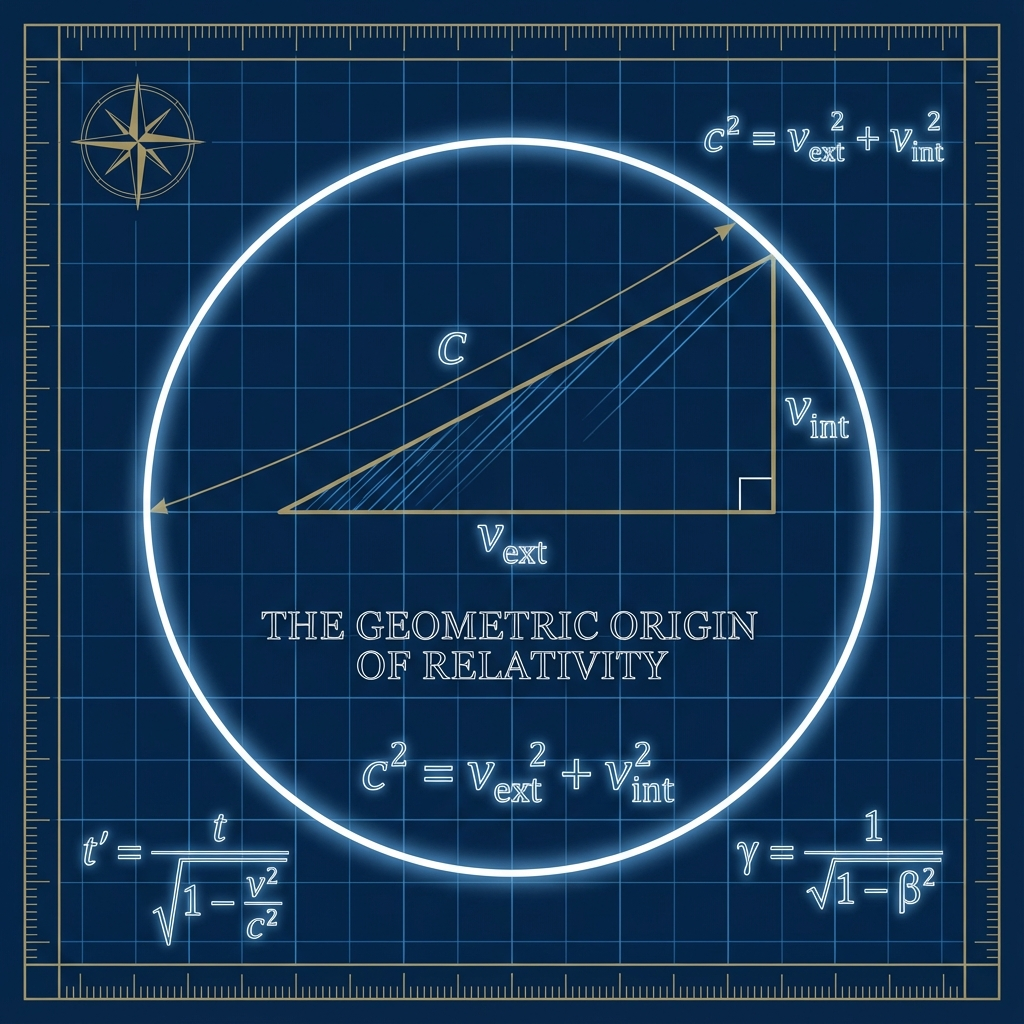
\includegraphics[width=0.8\textwidth]{assets/geometric_origin_of_relativity.png}
\caption{Geometric Evolution Circle}
\end{figure}


Let the cosmic state be a normalized vector $\psi(\tau)$ in Hilbert space. According to Axiom A1, its evolution rate is constant $c$:

$$||\dot{\psi}(\tau)||_{FS} = c$$

\section{Orthogonal Decomposition}

We introduce two orthogonal projection operators $P_{ext}$ (external/spatial sector) and $P_{int}$ (internal/temporal sector). According to Parseval's identity, the squared norm of the total evolution vector $V$ equals the sum of squared norms of its components:

$$v_{ext}^2 + v_{int}^2 = c^2 \quad \text{(A.1)}$$

where $v_{ext} = ||P_{ext}\dot{\psi}||_{FS}$, $v_{int} = ||P_{int}\dot{\psi}||_{FS}$. This is the mathematical form of the ``Great Trade-off'' in the main text.

\section{The Identification}

To establish connection with the physical world, we make the following natural mapping:

\begin{itemize}
\item \textbf{External velocity:} Identify $v_{ext}$ as the spatial coordinate velocity $v = \frac{dx}{dt}$.

\item \textbf{Internal velocity:} Identify $v_{int}$ as the rate of proper time ($\tau$) flow. For dimensional consistency, we set $v_{int} = c \frac{d\tau}{dt}$.
\end{itemize}

\section{Derivation of the Metric}

Substituting the above definitions into formula (A.1):

$$(\frac{dx}{dt})^2 + (c \frac{d\tau}{dt})^2 = c^2$$

Multiplying both sides by $dt^2$:

$$dx^2 + c^2 d\tau^2 = c^2 dt^2$$

Rearranging, we obtain the expression for proper time $\tau$:

$$c^2 d\tau^2 = c^2 dt^2 - dx^2 \quad \text{(A.2)}$$

Or written in line element form $ds^2 = -c^2 d\tau^2$ (using $-+++$ signature convention):

$$ds^2 = -c^2 dt^2 + dx^2$$

This is exactly the standard \textbf{Minkowski Line Element}. This shows that Lorentz symmetry is not an a priori geometric axiom, but a manifestation of isotropic evolution in Hilbert space under specific projections.

